% !TEX root = ../discriminative_filtering.tex

\section{Problem Description}
To filter neural data for use in BCI's, we must model the relationship between the neural data and the desired responses.  However, due to both physiological phenomena and engineering challenges, this relationship is constantly changing (nonstationary), sometimes over the course of mere hours~\cite{Per13,Per14}.  To overcome this problem, two types of solutions have been proposed in the literature: (1) incorporating frequent filter retraining to regularly update the model for this relationship and (2) developing new models that that can be trained to ignore small changes in this relationship.

\section{Approach I: Closed Loop Decoder Adaptation \index{Closed Loop Decoder Adaptation}}
Given a constant stream of new data, it is possible to retrain a filtering model at predetermined intervals.  This method requires establishing ground truth for the desired responses.  Any nonstationarity that develops must be present for some time (during which the decoder is presumably performing poorly) in order to catalog enough data so that it may be trained out at the next model refitting.  This method does not require the user to predict the nature of future nonstationarities and can adapt itself to drastic changes in the relationship between neural data and desired responses.  Researchers have demonstrated BCI filter robustness with this meta-approach using a wide variety of specific methods: adapting a discriminative Bayesian filter~\cite{Bra17}, refitting a Kalman filter~\cite{Gil12, Dan13}, Bayesian updating for an unscented Kalman filter~\cite{Li11}, reweighting a na\"ive Bayes classifier~\cite{Bis14}, retraining a kernelized ARMA model~\cite{Shp09}, and reinforcement learning~\cite{Mah13,Poh14}, among others.

\section{Approach II: Robust modeling}
Training a robust model presents a relatively less-explored but very promising solution to the problem of nonstationarities.  If changes in the relationship between neural data and desired response are predictable, then  a filter can be designed to effectively ignore the expected changes.  Such a filter can immediately adapt to small variability in this relationship and so does not require updating (or any feedback at all) in order to successfully decode in the presence of nonstationarities.  Because linear models (like those used in the Kalman filter) have limited expressiveness and tend to underfit rich datasets~\cite{Sus16}, we propose instead two powerful models from machine learning that can learn an arbitrary functional relationship between neural data and the desired responses: stateful recurrent neural networks (RNN's) and Gaussian Processes (GP's).

%%%%%%%%%%%%%%%%%%%%%%%%%%%%%%%%%%%%%%%%%%%%%%%%%
\begin{figure}[h]
\begin{minipage}[c]{.49\textwidth}
\caption[Data Augmentation]{Data augmentation. A. We iterate over each (neural,intention)-pair in our training set.  B. To protect against erratic behavior in the first dimension, we copy the (neural,intention)-pair, add noise to the first dimension, and add it to the training set with the same intention label.  We repeat this process, adding different random noise each time.  C. We repeat part (B) for each subsequent dimension in the neural space.  This process can increase the size of the training set by orders of magnitude.}
\end{minipage}
\hfill
\begin{minipage}[c]{.49\textwidth}
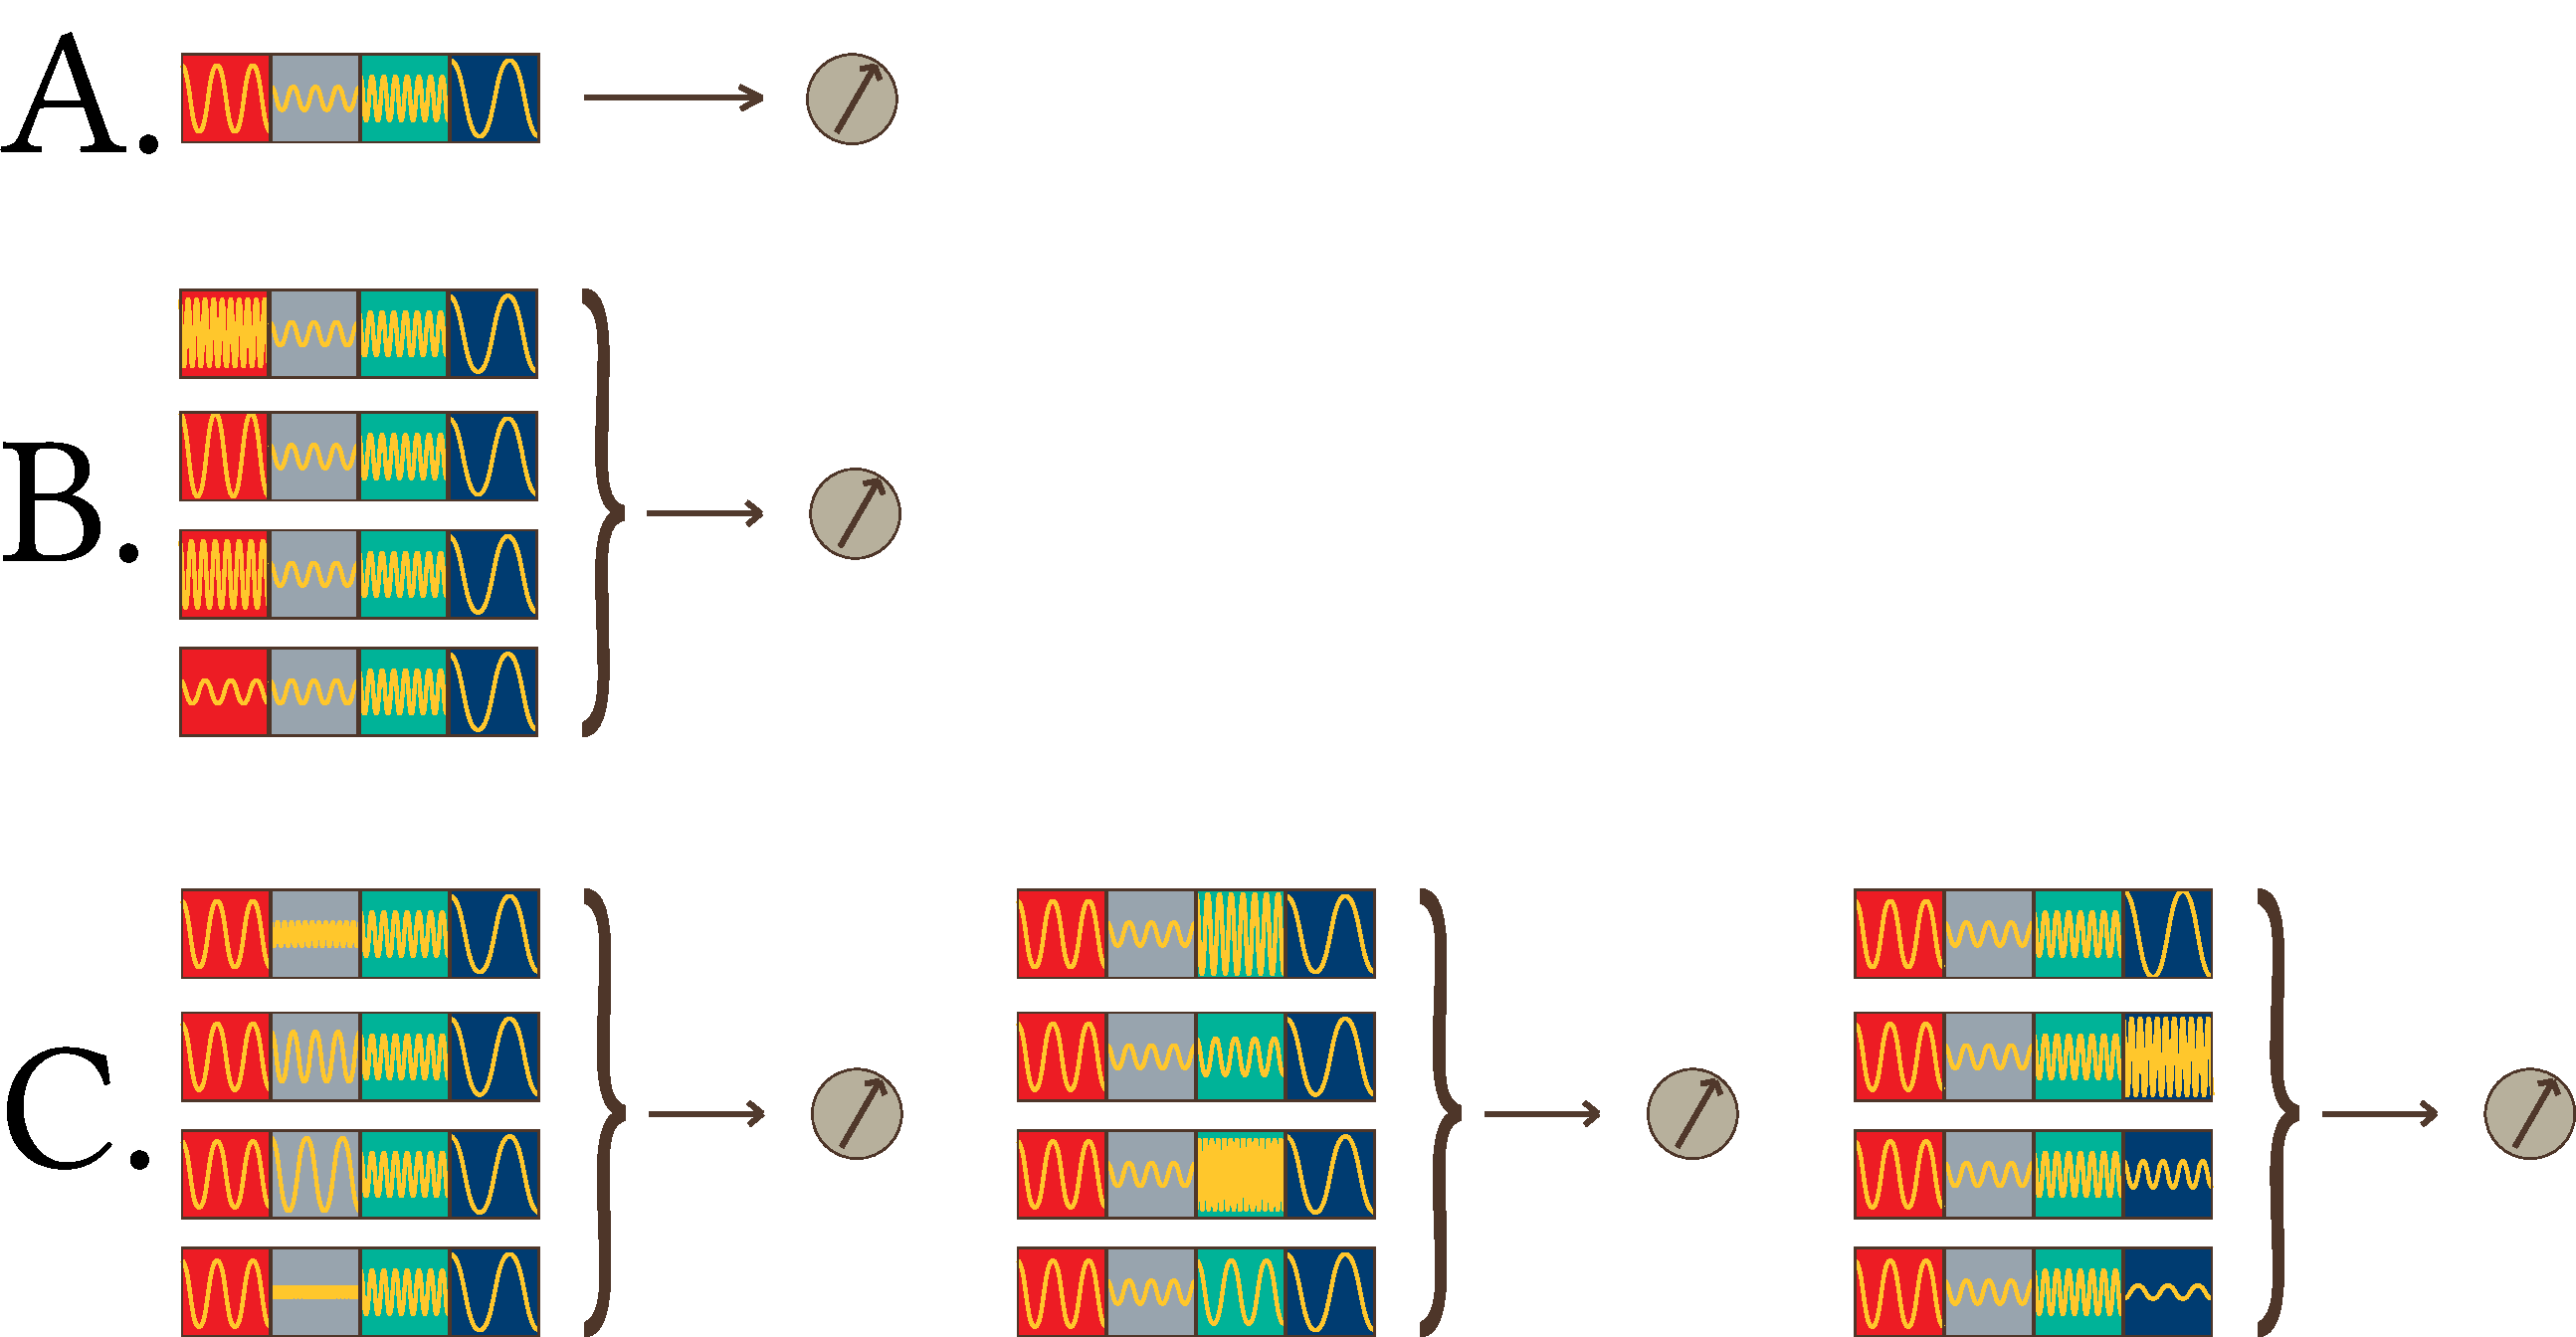
\includegraphics[width=\linewidth]{data_aug}
\end{minipage}
\index{neural networks!data augmentation} 
\end{figure}

\subsection{Stateful RNN's} 
Sussillo et al pioneered the training of fixed nonlinear BCI decoders for robustness in macaques~\cite{Sus16}.  To do so, they trained and successfully tested a multiplicative RNN-based neural filter.  Sussillo et al achieved robustness by augmenting their training data with perturbations that mimicked the desired nonstationities against which they wished to train.  For example, in order to train against dropping the $i$th neuron, they would add exemplars to their training set where firing from the $i$th neuron had been zeroed-out.  This technique of augmenting a training set with noisy data is well-established for increasing generalization performance in neural networks~\cite{An96}.  It requires generating and training over new artificial data for each individual nonstationarity they target.  In particular, the exemplars to protect against dropping the $i$th neuron do not protect against dropping the $j$th neuron.  Instead a new set of exemplars must be generated and trained on in order to achieve robustness for the $j$th neuron.  It is easy to see how this technique often enlarges an already massive dataset by orders of magnitude, entailing a commensurate increase in training burden for the neural network.

\subsection{GP's} 
In contrast to Sussillo, we achieve robustness through our choice of kernel, effectively altering the way we measure similarity between two firing patterns.  Given a new vector $z_t$ of neural features, the Gaussian process model predicts the mean inferred velocity $f(z_t)$ as a linear combination (\emph{cf}. \cite{Ras06} for an explanation):
\[
f(z_t) = \sum_{i=1}^n \alpha_i K_\theta(\zeta_i, z_t)
\]
where $\alpha := (K_\theta(\zeta,\zeta)+\theta_3^2I)^{-1}\chi$.  Thus the kernel $K_\theta$ evaluated on $\zeta_i$, $z_t$ directly determines the impact of the datapoint $(\zeta_i,\chi_i)$ on the prediction $f(z_t)$.  We choose a kernel that ignores large differences between $\zeta_i$ and $z_t$ if they occur along only a relatively few number of dimensions.  This makes our filter resilient to erratic firing patterns in an arbitrary single neuron (and presumably also in two or a few neurons, although we have not yet demonstrated this).  In particular, we do not need to handle dropping neuron $i$ and dropping neuron $j$ separately.  Altering our model to accommodate more or different nonstationarities would amount to a simple change in kernel and not result in increased training time. \index{Gaussian process regression!kernel selection} 

%%%%%%%%%%%%%%%%%%%%%%%%%%%%%%%%%%%%%%%%%%%%%%%%%
\begin{figure}[h]
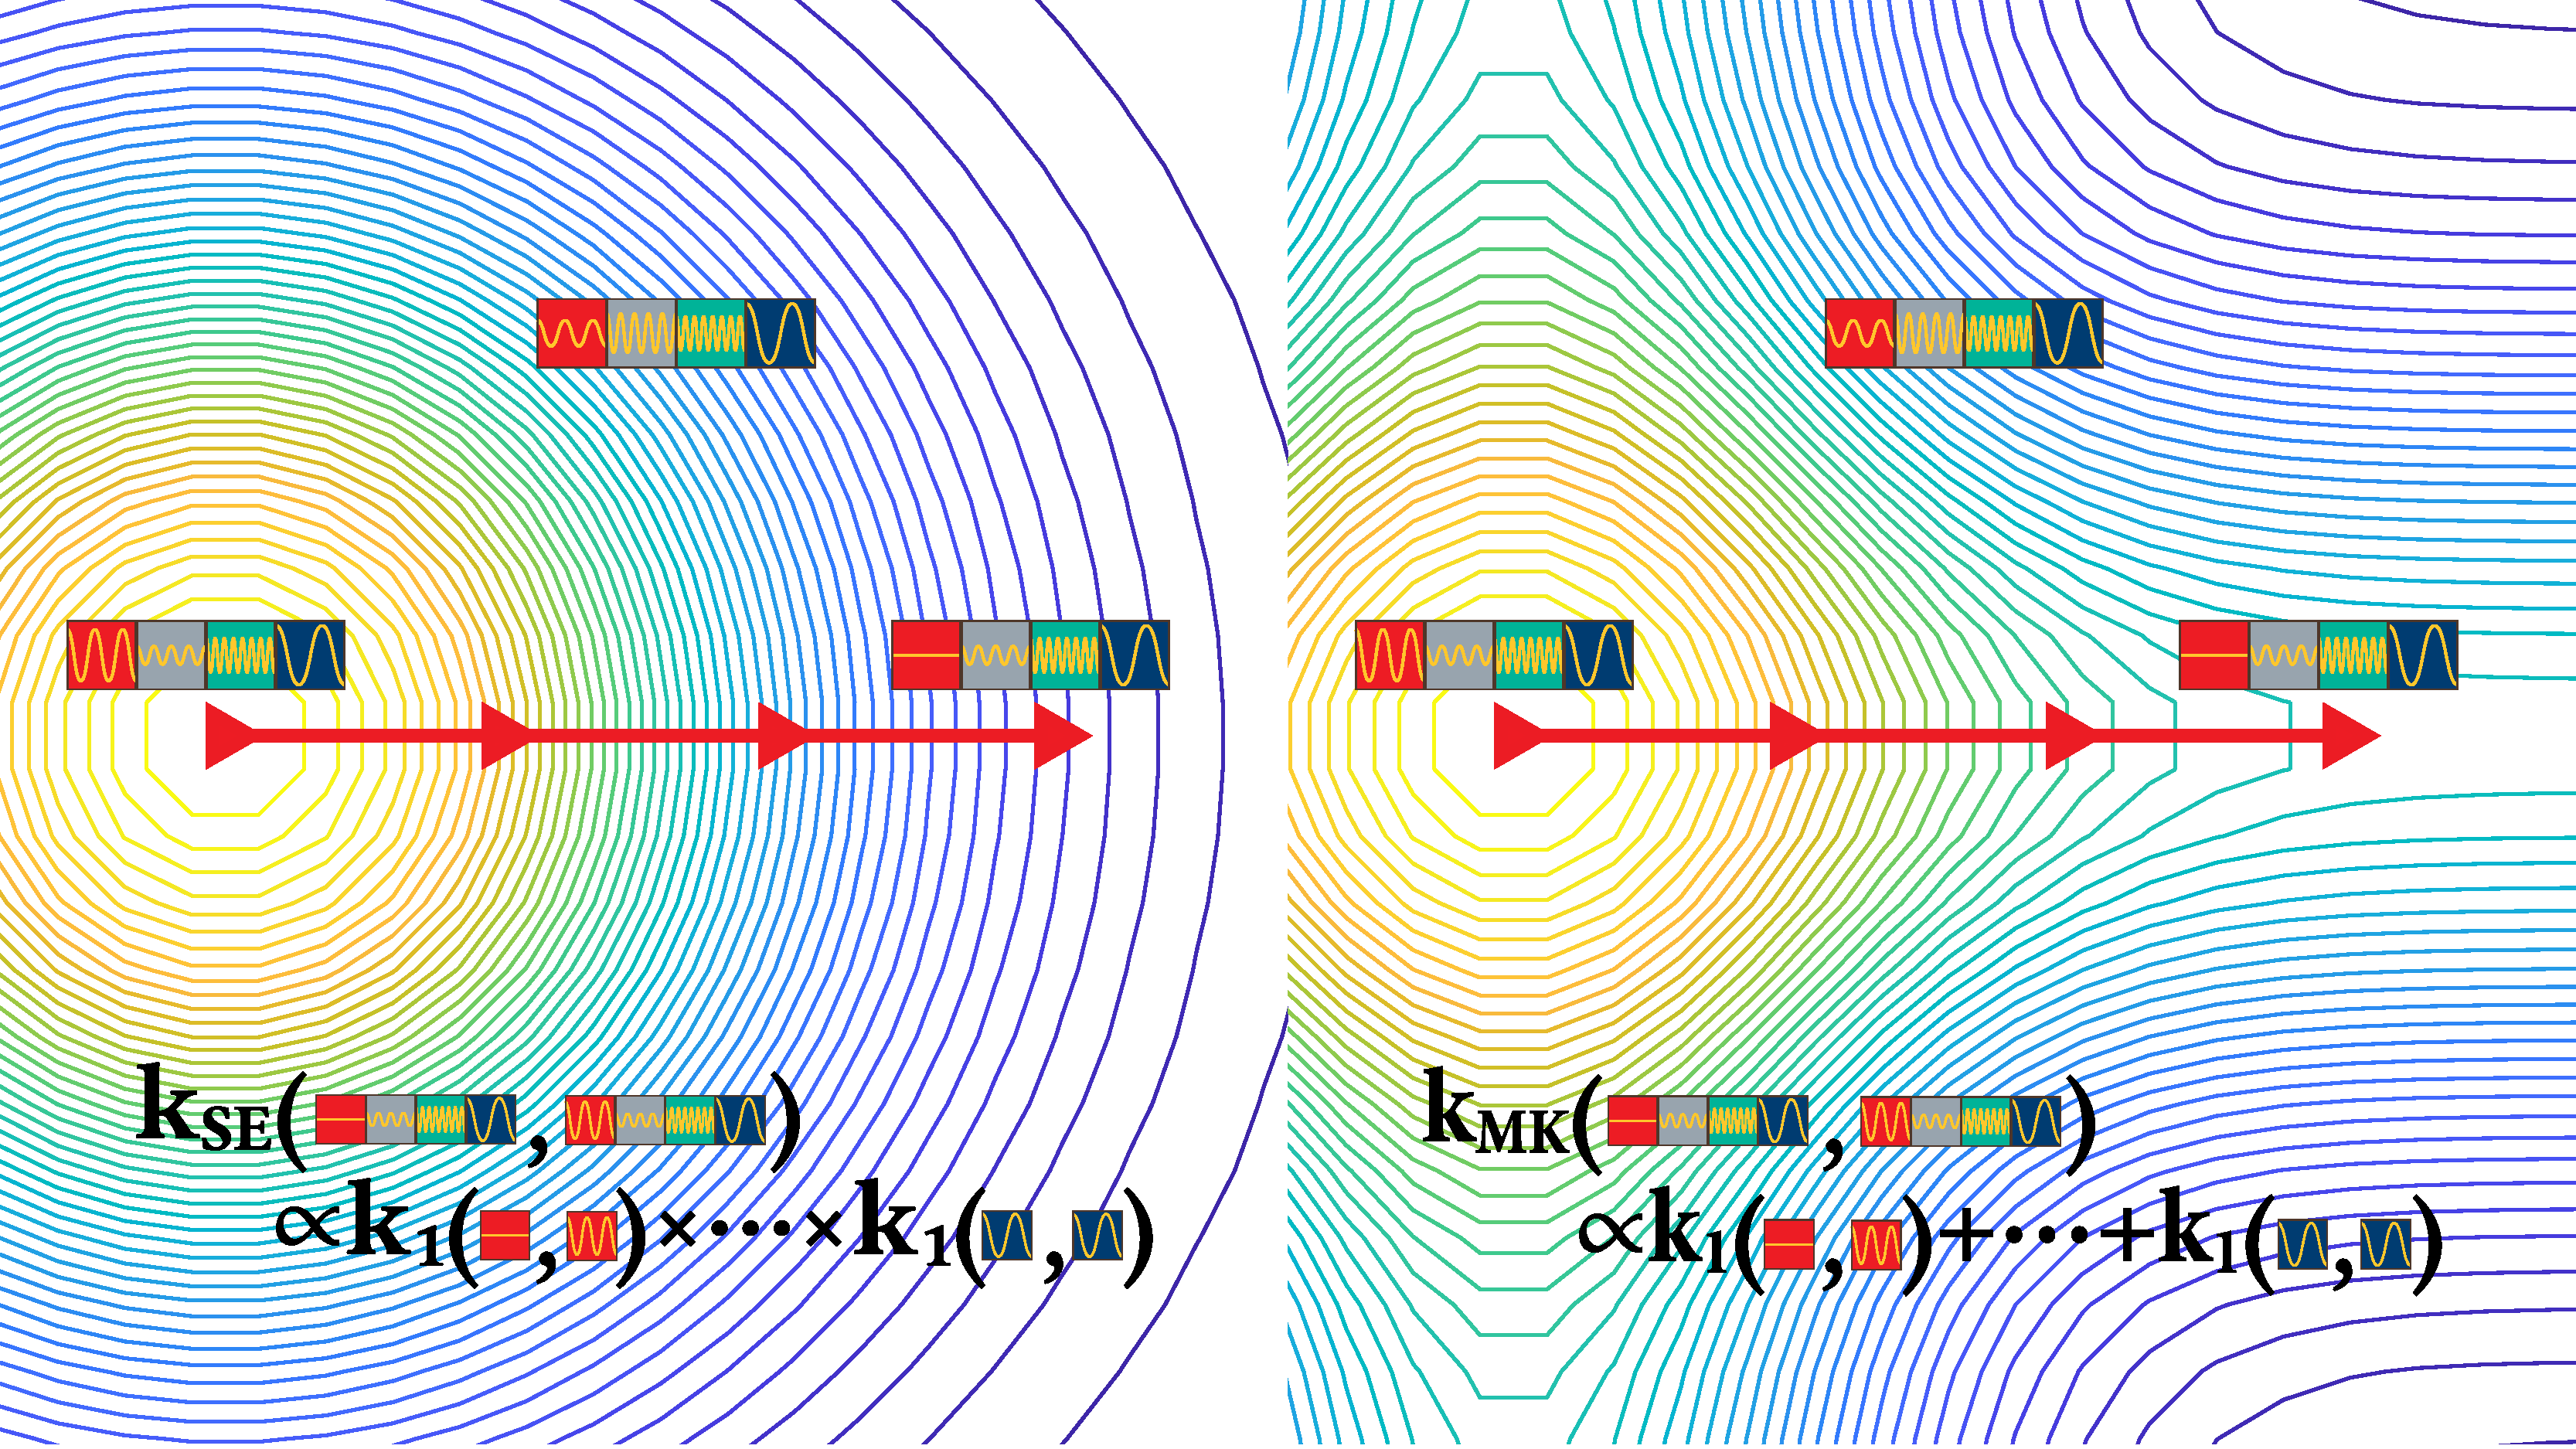
\includegraphics[width=\textwidth]{se_vs_mk}
\caption[Comparison of Squared Exponential and Multiple Kernels]{On the left, the squared exponential kernel calculates the similarity between two vectors as the geometric mean of the similarities along each dimension.  On the right, the multiple kernel calculates the similarity between two vectors as the arithmetic mean of the similarities along each dimension.  The multiple kernel approach limits the impact a single dimension can have on the determination of how similar two vectors are.}
\end{figure}

